We implemented the controller described in the previous section in order to regulate the height and roll of the water runner robot in simulation. The controller was tested against sinusoidal torques in the roll direction acting on the robot's body. To tune the gains on our virtual model, we used the Ziegler-Nichols Method as our virtual model is simply a PID controller in task-space. The last parameter $\omega_0$ was assigned according to a $50/50$ mix of the two averaging schemes outlined previously.

\begin{figure*}[t]
    \centering
    \begin{subfigure}[b]{0.49\textwidth}
        \centering
        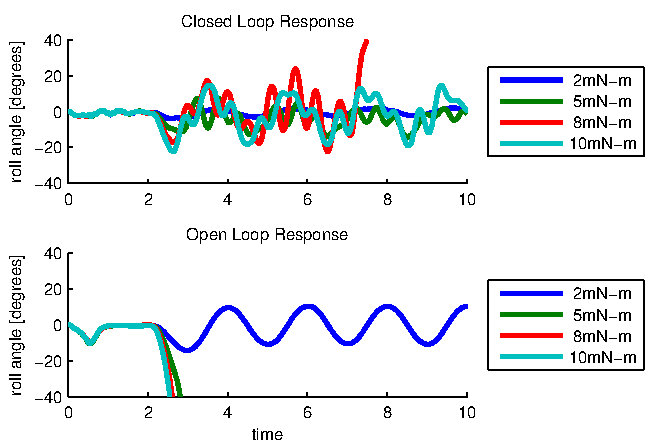
\includegraphics[width = \textwidth]{figures/torques_small.pdf}
        \caption{}
        \label{fig:results1Hz}
    \end{subfigure}
    \begin{subfigure}[b]{0.49\textwidth}
        \centering
        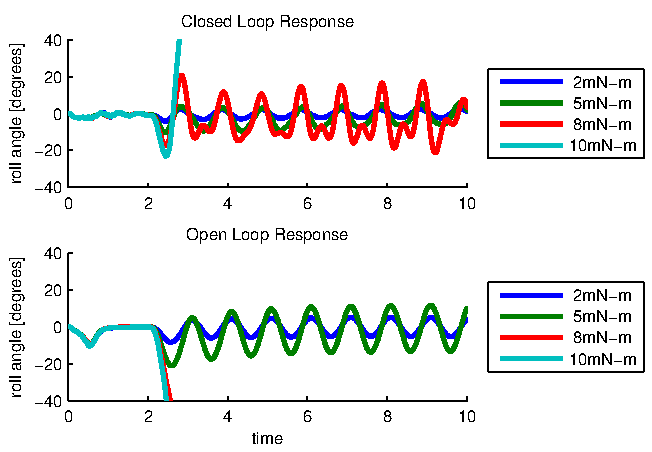
\includegraphics[width = \textwidth]{figures/torques_small2.pdf}
        \caption{}
        \label{fig:results2Hz}
    \end{subfigure}
    \caption{}
\end{figure*}

Figure~\ref{fig:results1Hz}
